%##############################################
\chapter{Theory and experimental status}
%##############################################

An introduction to the \gls{sm}, its particle content, interactions, and properties is provided in the following. Special focus is attributed to the top quark which is the heaviest known fundamental particle to date. Here, latest experimental results are discussed and the theoretical foundation of the measurements within this thesis is laid out.


%##############################################
\section{General quantum field theory of the Standard Model}
%##############################################

The \gls{sm} describes the interactions between fundamental particles. It is based on \gls{qft} which allows to predict observables of particle interactions. Exemplary observables are production cross sections or decay rates of particles which can be calculated within its framework -- even fully automatized. The \gls{sm} validity is constantly challenged by comparing predictions to experimental data. No significant deviations have been found so far that would hint towards physics \gls{bsm}.


%##############################################
\subsection{Particle content}
%##############################################

Fundamental particles are objects for which experiments have revealed no internal structure. For example, only an upper limit on the spatial radius of an electron has been measured to be $<10^{-18}~\mathrm{m}$~\cite{PhysRevLett.97.030801}. Such particles are therefore considered as point-like. Fundamental particles can be grouped by their spin into fermions with spin~$\frac{1}{2}$ and bosons with integer spin. The fermions can be further divided into leptons and quarks where only the later can participate in strong interactions. Tables~\ref{tab:theory-leptons} and~\ref{tab:theory-quarks} list the leptons and quarks respectively. Each column is called a generation. It encapsulates an isospin pair whose components are therefore also referred to as up- or down-type respectively. It is unknown why there are exactly three lepton and three quark generations. Ordinary atoms consists of only particles from the first generator: electron, proton~p~(uud quarks) and neutron~n~(udd quarks).\todo{mention searches for 4th generation?}

\mytable{\label{tab:theory-leptons}Leptons of the \gls{sm}. Particle masses are taken from Ref.~\cite{Olive:2016xmw}. Uncertainties on the measured masses are omitted because the precision is beyond the sub permille level. For the neutrino masses only \glspl{cl} are given.}{
\begin{tabular}{r||c|c|c}
                        & 1. generation                 & 2. generation                 & 3. generation \\
    \hline
    \hline
    name                & electron ($\mathrm{e}^{\rmminus}$)   & muon ($\mu^{\rmminus}$)              & tau ($\tau^{\rmminus}$) \\
    \hline
    mass                & $511.0~\keV$                  & $105.66~\MeV$                 & $1.776~\GeV$ \\
    \hline
    electric charge     & $-1$                          & $-1$                          & $-1$ \\
    \hline
    \hline
    name                & electron neutrino             & muon neutrino                 & tau neutrino  \\
                        & ($\nu_\mathrm{e}$)            & ($\nu_{\mu}$)                 & ($\nu_{\tau}$) \\
    \hline
    mass                & $<225~\eV$                    & $<0.19~\MeV$                  & $<18.2~\MeV$ \\
                        & (95\% CL)                     & (90\% CL)                     & (95\%~CL)\\
    \hline
    electric charge     & 0                             & 0                             & 0 \\
    \end{tabular}
}

For the neutrinos masses, only upper limits on their masses are given. Those are derived by combining measurements of beta decay kinematics with results from neutrino oscillation experiments. In the \gls{sm}, neutrinos are assumed to be massless. However, the observation \todo{need ref} of neutrino oscillations requires that at least two neutrinos have a non-zero mass.

\mytable{\label{tab:theory-quarks}Quarks of the \gls{sm}. For u,d,s,c,b quarks, \msbar masses are taken from Ref.~\cite{Olive:2016xmw}. The top quark pole mass is taken from Ref.~\cite{ATLAS:2014wva}.}{
\begin{tabular}{r||c|c|c}
                        & 1. generation                 & 2. generation                 & 3. generation \\
    \hline
    \hline
    name                & up (u)                        & charm (c)                     & top (t) \\
    \hline
    mass                & $2.2^{+0.6}_{-0.4}~\MeV$      & $1.27\pm0.03~\GeV$            & $173.34\pm0.71~\GeV$ \\
    \hline
    electric charge     & $\frac{2}{3}$                 & $\frac{2}{3}$                 & $\frac{2}{3}$ \\
    \hline
    \hline
    name                & down (d)                      & strange (s)                   & bottom (b)  \\
    \hline
    mass                & $4.7^{+0.5}_{-0.4}~\MeV$      & $96^{+8}_{-4}~\MeV$           & $4.18^{+0.04}_{-0.03}~\GeV$ \\
    \hline
    electric charge     & $-\frac{1}{3}$                & $-\frac{1}{3}$                & $-\frac{1}{3}$ \\

    \end{tabular}
}


The bosons are connected to fundamental interactions by requiring invariance under a gauge group transformation as explained later in this chapter. They are listed in Tab.~\ref{tab:theory-bosons}. All bosons except the Higgs boson carry a spin of~$1$. The Higgs boson is the only scalar particle~(spin~$0$) of the \gls{sm}. For a long time, it was a purely hypothetical particle of the \gls{sm}. In July 2012, the ATLAS~\cite{Aad:2012tfa} and CMS~\cite{Chatrchyan:2012xdj} collaborations independently reported an observation of a Higgs-like particle. Further investigations whether this new particle exhibits the expected interactions with other particles revealed that it is consistent with the \gls{sm} Higgs~\cite{Khachatryan:2016vau} boson. This discovery completed the \gls{sm} and thus gave further confidence into its theoretical footing.


\mytable{\label{tab:theory-bosons}Bosons of the \gls{sm}. Z and W boson masses are taken from Ref.~\cite{Olive:2016xmw}. The uncertainties on their masses are omitted because the precision is beyond the sub permille level. The Higgs mass is taken from Ref.~\cite{Aad:2015zhl}.}{
\begin{tabular}{r||c|c|c}
    name                & mass                 & associated interaction             & gauge group \\
    \hline
    \hline
    photon (\photon)    & $0$                  & electromagnetism                   & $\mathrm{U(1)}$ \\
    \hline
    Z boson (\zboson)   & $91.19~\GeV$         & \multirow{2}{*}{weak interaction}  & \multirow{2}{*}{$\mathrm{SU(2)}$}\\
    W boson (\wboson)   & $80.39~\GeV$         &                                    & \\
    \hline
    Higgs boson (\higgs)& $125.09\pm0.24~\GeV$ & Yukawa interaction                 & $\mathrm{U(1)}$\\
    \hline  
    8 gluons (g)        & $0$                  & strong interaction                 & $\mathrm{SU(3)}$ \\                 
    \end{tabular}
}

Each fundamental particle has additionally a charge-conjugated partner called antiparticle. Other properties such as mass are identical. The photon, Z boson, and Higgs boson are their own antiparticle. It is still under study if the neutrino is its own antiparticle. Fermions with such a property are called Majorana particles~\cite{Majorana2006}. Experimentally, this can be probed in double $\beta$ decays~($\mathrm{nn}\to\mathrm{pp}+\mathrm{e}^{\rmminus}\mathrm{e}^{\rmminus}\nu_\mathrm{e}\nu_\mathrm{e}$) where in the case of Majorana neutrinos the decay can occur without emitting two neutrinos. However, this scenario seems to be disfavored by recent results as reviewed in Ref.~\cite{Dell'Oro:2016dbc}.


%##############################################
\subsection{Quantum field theory}
%##############################################

In the framework of \gls{qft}, particles are described as excitation modes of quantized fields. This is also referred to as ``second quantization'' allowing to describe many-particle systems. Field operators can be decomposed as

\begin{align}
    \hat{\psi}(x)&=\sum_{i}^{\mathrm{N}}u_{i}(x)\hat{a}_{i} \\
    \hat{\psi}^{\dagger}(x)&=\sum_{i}^{\mathrm{N}}u^{\star}_{i}(x)\hat{a}^{\dagger}_{i},
\end{align}

where $u_{i}(x)$ denotes the ordinary wave function of a single particle and $\hat{a}^{\dagger}_{i}$ ($\hat{a}_{i}$) its creation (annihilation) operator, respectively.

As in classical mechanics, the action of a system can be expressed as

\begin{equation}
S=\int\mathrm{L}\,\mathrm{d}t=\iint\mathcal{L}\,\mathrm{d}^{3}\vec{x}\,\mathrm{dt}=\int\mathcal{L}\,\mathrm{d}^{4}x
\end{equation}

with the Lagrangian density $\mathcal{L}$. For example, a system of free fermions is described by the Dirac Lagrangian density,

\begin{equation}
\label{eq:theory-diracL}
\mathcal{L}_\mathrm{Dirac}=\bar{\psi}\big(i\gamma^\mu\partial_\mu-m\big)\psi
\end{equation}

using the definitions $\partial_\mu\equiv\partial/\partial x_\mu$ and $\bar{\psi}\equiv\psi^\dagger\gamma^{0}$ where $\gamma_\mu$ denote the Dirac matrices\footnote{Multiple representations are possible. The matrices need to satisfy a Clifford algebra with the anticommutation relation: $\big\{\gamma^\mu,\gamma^\nu\big\}=\gamma^\mu\gamma^\nu+\gamma^\nu\gamma^\mu=2g^{\mu\nu}$.}. The principle of least action, $\delta \mathrm{S}=0$, that is satisfied by the Euler-Lagrange equation yields the equation of motion as

\begin{equation}
\frac{\partial\mathcal{L}}{\partial\bar{\psi}}-\frac{\partial}{\partial_\mu}\Bigg(\frac{\partial\mathcal{L}}{\partial\big(\partial_\mu\bar{\psi}\big)}\Bigg)=\big(i\gamma^\mu\partial_\mu-m\big)\psi=0. \\
\end{equation}

Assuming $\psi\propto e^{-ip^{\mu}x_{\mu}}$ leads directly to the well-known energy-momentum relation

\begin{align}
0&=\big(i\gamma^\mu\partial_\mu-m\big)\cdot \big(-i\gamma^\nu\partial_\nu-m\big)\psi\\
 &=\big(\partial^{\mu}\partial_{\mu}+m^{2}\big)\psi \qquad \mathrm{(``Klein\mbox{-}Gordan''~equation)}  \\
 &\Rightarrow \big(-p^{\mu}p_{\mu}+m^{2}\big) = 0.
\end{align}


In the \gls{sm}, interactions between particles are introduced by requiring local invariance of the Lagrangian density for certain groups of gauge transformations. In the following, this is briefly demonstrated for the case of a $\mathrm{U(1)}$ transformation which leads to electromagnetic interactions.

The transformation of Eq.~\ref{eq:theory-diracL} using 

\begin{equation}
\psi(x)\mapsto\psi^{\prime}(x)=\psi\exp^{-iq\alpha(x)}
\end{equation}

where the phase $\alpha(x)$ depends on the local coordinates $x$ yields

\begin{equation}
\mathcal{L}(\psi,\partial_\mu\psi)\mapsto\mathcal{L}(\psi^{\prime},\partial_\mu\psi^{\prime})=\bar{\psi}\big(i\gamma^\mu\partial_\mu+q\gamma^\mu\partial_\mu\alpha(x)-m\big)\psi.
\end{equation}

The invariance $\mathcal{L}(\psi,\partial_\mu\psi)=\mathcal{L}(\psi^{\prime},\partial_\mu\psi^{\prime})$ is restored by adding a bosonic spin-1 field $A_{\mu}(x)$ which interacts with $\psi$ while transforming as

\begin{equation}
A_{\mu}(x)\mapsto A^{\prime}_{\mu}(x)=A_\mu(x)-\partial_\mu\alpha(x).
\end{equation}

This procedure yields a Lagrangian density containing the following terms:

\begin{align}
\mathcal{L}=~~&\bar{\psi}\big(i\gamma^\mu\partial_\mu-m\big)\psi &(\mathrm{fermion~propagator}) \\
            +&q\bar{\psi}\gamma^{\mu}\psi A_{\mu} &(\mathrm{interaction}) \label{eq:theory-EM-int}\\
            -&\tfrac{1}{4}\big(\partial_\mu A_\nu-\partial_\nu A_\mu\big)^{2} &(\mathrm{boson~propagator})
\end{align}

The boson propagator describing the dynamics of a free $A_\mu$ field has been added additionally to the Lagrangian density. It is already invariant under the local gauge transformation. The introduced interaction~(Eq.~\ref{eq:theory-EM-int}) which is required to ensure the invariance under $\mathrm{U(1)}$ transformation can be identified as electromagnetic interaction between a fermion described by $\psi$ with electric charge $q$ and a photon described by $A_\mu$. Furthermore, the photon is predicted to be massless since adding a term of the form $m^{2}_{A}A^\mu A_\mu$ would violate the invariance.

Other interactions of the \gls{sm} are also connected to local gauge transformations which can be introduced through similar procedures. A common property follows from the Noether theorem which states that for each continuous transformation a conserved current exists. Hence the charge associated to each gauge group is conserved. This would however be already the case for a global transformation. The requirement of invariance under an even local gauge transformations is a puzzling feature of the theory. \todo{ref to some philosophical arguments? is there an implication from renormalization?}

%##############################################
\subsection{Electroweak interactions and Higgs mechanism}
%##############################################
\label{sec:theory-ewk}

Electromagnetic and weak interactions can be unified using a $\mathrm{U(1)}\otimes \mathrm{SU(2)}$ gauge group. Furthermore, the theory needs to account for the following features found experimentally.

\begin{itemize}

\item Parity is not conserved in weak interactions. Such interactions depend on the spin being aligned towards or against the momentum of a particle. Experimentally, the Wu experiment~\cite{PhysRev.105.1413} discovered this feature in ${}_{27}^{60}\mathrm{Co}\to{}_{28}^{60}\mathrm{Ni}+e^{\rmminus}\bar{\nu}_{e}\gamma\gamma$ decays by analyzing the direction of the electron with respect to the polarization of the cobalt probe through an external magnetic field. 

\item The UA1 and UA2 experiments at the CERN SPS proton-antiproton collider discovered that \wboson bosons~\cite{Arnison:1983rp,Banner:1983jy} and \zboson bosons~\cite{Arnison:1983mk,Bagnaia:1983zx} -- mediators of weak interactions -- are massive. The masses of these particles have to be introduced in a different way if the concept of local gauge invariance should continue to hold.

\end{itemize}

To account for the violation of parity, fermion fields have to be first decomposed into chiral eigenstates using the projections

\begin{align}
\psi_\mathrm{L}&\equiv\mathrm{P}_\mathrm{L}\psi=\tfrac{1}{2}(1-\gamma_{5})\psi \\
\psi_\mathrm{R}&\equiv\mathrm{P}_\mathrm{R}\psi=\tfrac{1}{2}(1+\gamma_{5})\psi
\end{align}

with $\gamma_{5}=i\gamma_{0}\gamma_{1}\gamma_{2}\gamma_{3}$\footnote{Properties: $(\gamma_{5})^{\dagger}=\gamma_{5}$; ~~$(\gamma_{5})^2=\mathrm{I}_\mathrm{4x4}$; ~~ $\{\gamma_{5},\gamma_{\mu}\}=\gamma_{5}\gamma_{\mu}+\gamma_{\mu}\gamma_{5}=0$.} where $\psi_\mathrm{L}$ ($\psi_\mathrm{R}$) is called ``left-handed'' (``right-handed'') respectively. In the case of massless particles, Eq.~\ref{eq:theory-diracL} decouples into two independent equations for $\psi_\mathrm{L}$ and $\psi_\mathrm{R}$. Here, the chirality is equal to the Lorentz-invariant helicity

\begin{equation}
\mathrm{H}\equiv\frac{\vec{p}\cdot\vec{s}}{|\vec{p}|}
\end{equation}

which denotes whether the spin $\vec{s}$ is aligned along~($H=1$) or against~($H=-1$) the momentum axis. For massive particles, Eq.~\ref{eq:theory-diracL} cannot be decomposed since chirality is not Lorentz invariant. \todo{CP is violated}\todo{add that CPT is considered invariant}

The Glawhow-Weinberg-Salam model~\cite{Salam:1964ry,Weinberg:1967tq,Glashow:1961tr} splits the fermion fields into ``left-handed'' doublets 

\begin{align}
\vec{\mathrm{E}}_\mathrm{L}&=\Bigg\{\colvec{2}{\nu_\mathrm{e,L}}{e^{\rmminus}_\mathrm{L}},\colvec{2}{\nu_{\mu,\mathrm{L}}}{\mu^{\rmminus}_\mathrm{L}},\colvec{2}{\nu_{\tau,\mathrm{L}}}{\tau^{\rmminus}_\mathrm{L}}\Bigg\} \label{eq:theory-su2-leptons} \\
\vec{\mathrm{Q}}_\mathrm{L}&=\Bigg\{\colvec{2}{\mathrm{u}_\mathrm{L}}{\mathrm{d}_\mathrm{L}},\colvec{2}{\mathrm{c}_\mathrm{L}}{\mathrm{s}_\mathrm{L}},\colvec{2}{\mathrm{t}_\mathrm{L}}{\mathrm{b}_\mathrm{L}}\Bigg\} \label{eq:theory-su2-quarks}
\end{align}

and ``right-handed'' singlets 

\begin{align}
\vec{\mathrm{e}}_\mathrm{R}=\big\{\mathrm{e}^{\rmminus}_\mathrm{R},\mu^{\rmminus}_\mathrm{R},\tau^{\rmminus}_\mathrm{R}\big\},\quad\vec{\mathrm{u}}_\mathrm{R}=\big\{\mathrm{u}_\mathrm{R},\mathrm{c}_\mathrm{R},\mathrm{t}_\mathrm{R}\big\},\quad\vec{\mathrm{d}}_\mathrm{R}=\big\{\mathrm{d}_\mathrm{R},\mathrm{s}_\mathrm{R},\mathrm{b}_\mathrm{R}\big\}
\end{align}

of the $\mathrm{SU(2)}$ group. Right-handed neutrinos do not participate in any interaction within the \gls{sm}\todo{they could if massive?}. The gauge transformation of the combined group is

\begin{equation}
\psi\mapsto\psi\cdot\mathrm{e}^{-ig\vec{\alpha}(x)\cdot\vec{\omega}/2}\cdot\mathrm{e}^{-ig^{\prime}\beta(x)/2} \label{eq:theory-u1su2-transformation}
\end{equation}

where $\omega_{a}$~($a\in\{1,2,3\}$) denote the Pauli matrices and $g$, $g^{\prime}$ the corresponding conserved charges. This leads to four boson fields, $W^{a}_{\mu}$ and $B_{\mu}$, that interact with the fermions. Hence in analogy to Eq.~\ref{eq:theory-EM-int} one obtains

\begin{align}
\mathcal{L}_\mathrm{interaction}=~~\sum_{\psi_\mathrm{L}}^\mathrm{doublets}&\bar{\psi}^{i}_\mathrm{L}~\gamma^{\mu}\big(\tfrac{1}{2}g\vec{W}_{\mu}\cdot\vec{\omega}+\tfrac{1}{2}g^{\prime}B_{\mu}\big)\psi^{i}_\mathrm{L} \\
+\sum_{\psi^{i}_\mathrm{R}}^\mathrm{singlets}&\bar{\psi}^{i}_\mathrm{R}~\gamma^{\mu}\tfrac{1}{2}g^{\prime}B_{\mu}\psi^{i}_\mathrm{R} + \mathrm{\gls{hc}}
\end{align}
\todo{is it correct that singlets do not couple to A?}

where the summation is implied over the fermion doublets and singlets. The coupling structure $\propto(\gamma_{\mu}-\gamma_{\mu}\gamma_{5})$ between $W_{\mu}^{a}$ and $\psi$ is called a \gls{va} structure because of its spatial transformation properties. \todo{elaborate more! e.g. antiparticle} and obeys the observation of the Wu experiment.

Unfortunately, a fermion mass term $\propto m_\mathrm{f}\bar{\psi}_\mathrm{f}\psi_\mathrm{f}=m_\mathrm{f}(\bar{\psi}_\mathrm{f,L}\psi_\mathrm{f,R}+\bar{\psi}_\mathrm{f,R}\psi_\mathrm{f,L})$ cannot be added to the Lagrangian density since it is not invariant under $\mathrm{SU(2)}$ transformation. To introduce mass terms for fermions and the \wboson/\zboson gauge bosons, a solution is provided by the Englert-Brout-Higgs-Guralnik-Hagen-Kibble-mechanism~\cite{HIGGS1964132,PhysRevLett.13.508,PhysRevLett.13.321,PhysRevLett.13.585}. A new scalar $\mathrm{SU(2)}$ doublet field $\phi=(\phi^{\rmplus},\phi^{0})$\footnote{$\phi^{\rmplus}$ annihilates positively charge scalar particles / creates antiparticles with negative charge; $\phi^{0}$ annihilates neutral particles / creates neutral antiparticles.} -- invariant under $\mathrm{U(1)}\otimes\mathrm{SU(2)}$ -- is added to the Lagrangian density

\begin{align}
\mathcal{L}_{\phi}&=\big(D_{\mu}\phi^{\dagger}\big)\big(D^{\mu}\phi\big)+\mathrm{V}(\phi) \label{eq:theory-phi-propagator} \\
D^{\mu}\phi&=\big(\partial^{\mu}+\tfrac{1}{2}ig\vec{W}^{\mu}\cdot\vec{\omega}+\tfrac{1}{2}ig^{\prime}B^{\mu}\big)\phi \label{eq:theory-phi-codev}
\end{align}

which interacts with the gauge bosons. In addition, $\phi$ has a potential 

\begin{equation}
\mathrm{V}(\phi)=-\mu^2\phi^\dagger\phi+\tfrac{1}{2}\lambda(\phi^\dagger\phi)^2
\end{equation}

in the form of a ``Mexcian hat'' as shown in Fig.~\ref{fig:theory-higgs-potential} that leads to a \gls{vev} of $\phi_0=\sqrt{\mu^{2}/\lambda}\equiv v/\sqrt{2}$ for $\mu^2>0$.

\myfigure{\label{fig:theory-higgs-potential}The ``Mexican hat'' potential of the Higgs field with a non-zero \gls{vev} $\phi_0$ which leads to symmetry breaking.}{
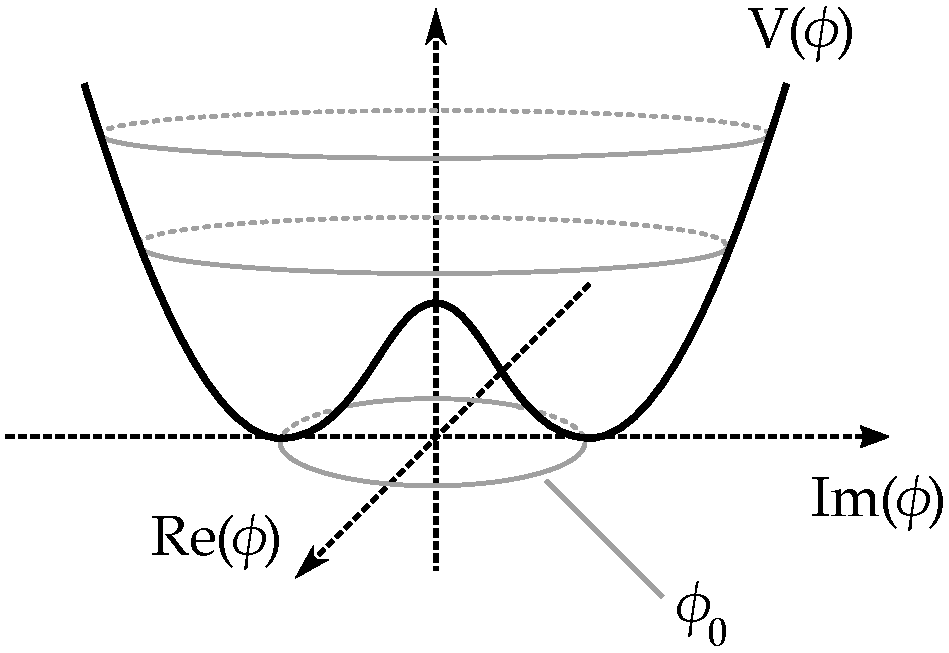
\includegraphics[width=0.5\textwidth]{figures/theory/higgspot.pdf}
}

One says that this shifted \gls{vev} ``breaks'' the $\mathrm{SU(2)}$ symmetry when parameterizing $\phi$ around the minimum as

\begin{equation}
\phi(x) \big|_{\phi_0} = \colvec{2}{0}{\frac{1}{\sqrt{2}}\big(v+h(x)\big)}\cdot \mathrm{e}^{-i\vec{\theta}(x)\cdot\vec{\omega}/(2v)} \label{eq:theory-phi-dev}
\end{equation}

where $\vec{\theta}$ denotes three so-called ``Goldstone'' bosons and $h$ the Higgs boson. In fact, the symmetry still exists but is ``hidden''. A $\mathrm{SU(2)}$ transformation, called ``unitary'' gauge, can be performed such that $\vec{\theta}$ vanishes. One says that these three Goldstone bosons and their degrees of freedom are ``eaten'' by the \wboson and \zboson bosons to become massive and hence can have also a longitudinal polarization. After the gauge transformation, the Higgs boson remains. The parametrization is chosen such that it leaves the minimum invariant under the $\mathrm{U(1)}$ transformation

\begin{equation}
\phi\mapsto\phi\cdot\mathrm{e}^{-ig\alpha_{3}(x)\omega_{3}/2}\cdot\mathrm{e}^{-ig^{\prime}\beta(x)/2}. \label{eq:theory-broken-u1-trans}
\end{equation}

Inserting Eq.~\ref{eq:theory-phi-dev} into Eq.~\ref{eq:theory-phi-propagator} yields the following non-interaction terms

\begin{align}
\mathcal{L}_\mathrm{Higgs}&=~~~\tfrac{1}{2}(\partial_{\mu}h^{\dagger})(\partial^{\mu}h)-\lambda^2 v^2 h^2 \label{eq:theory-higgs} \\
\mathcal{L}_\mathrm{W_1,W_2~bosons}&=-\tfrac{1}{8}g^2 v^2 \big(W_{1,\mu} W_{1}^{\mu}+W_{2,\mu} W_{2}^{\mu}\big) \label{eq:theory-a1a2} \\
\mathcal{L}_\mathrm{W_3,B~bosons}&=-\tfrac{1}{8}v^2 \big(gW_{3,\mu}-g^{\prime}B_\mu\big)\big(gW_{3}^{\mu}-g^{\prime}B^\mu\big) \label{eq:theory-a3b}.
\end{align}

The first term (Eq.~\ref{eq:theory-higgs}) describes a free scalar boson, the Higgs boson \higgs, with mass $m=\lambda v$. Next, the $W_{1}$ and $W_{2}$
fields in Eq.~\ref{eq:theory-a1a2} can be identified as a particle/antiparticle pair $\wboson=1/\sqrt{2}(W_1\mp iW_2)$ with mass $m_{\wboson}=\frac{1}{2}gv$. Lastly, the fields $W_3$ and $B$ appear to be in a mixed mass state~(Eq.~\ref{eq:theory-a3b}). By performing a rotation of the couplings

\begin{equation}
\colvec{2}{\zboson}{A}=\begin{pmatrix}
\cos\theta_\mathrm{W} & -\sin\theta_\mathrm{W} \\
\sin\theta_\mathrm{W} & \cos\theta_\mathrm{W}
\end{pmatrix}
\colvec{2}{W_{3}}{B},\quad \cos\theta_\mathrm{W}=\frac{g}{\sqrt{g^2+g^{\prime 2}}},
\end{equation}

where $\theta_\mathrm{W}$ is called the ``weak-mixing'' or ``Weinberg'' angle, another massive boson $\zboson$ with mass $m_\zboson=v\sqrt{g^2+g^{\prime2}}/2$ and a massless boson $A_\mu$, the photon, can be identified. The angle is determined as $\sin^2\theta_\mathrm{W} \approx 0.2312$ through the mass ratio $m_\wboson/m_\zboson=\cos\theta_\mathrm{W}$. Rewriting the covariant derivative of Eq.~\ref{eq:theory-phi-codev} into these mass eigenstates yields

\begin{align}
\mathcal{L}=&~~~~\partial_\mu+i\frac{g}{\sqrt{2}}\cdot\big(W^{\rmplus}_\mu T^{\rmplus}+W^{\rmminus}_\mu T^{\rmminus})\\
&-i\frac{g^2T_3-g^{\prime 2}Y}{\sqrt{g^2+g^{\prime 2}}}\cdot\zboson_\mu-i\frac{g^{\prime}g\big(T^3+Y\big)}{\sqrt{g^2+g^{\prime 2}}}\cdot A_\mu
\end{align}

where $T^{\pm}$ denote the ladder operators, $Y$ the $\mathrm{U(1)}$ so-called ``hyper'' charge and $T_3$ the $\mathrm{SU(2)}$  charge. From the coupling to the photon one can read of the electric coupling constant to be 

\begin{equation}
e=\frac{g^{\prime} g}{\sqrt{g^2+g^{\prime 2}}}~,\quad \aem=\frac{e^2}{4\pi}=\frac{1}{137}
\end{equation}

and the corresponding electric charge to be $Q=T_3+Y$ which is invariant under Eq.~\ref{eq:theory-broken-u1-trans}. For the weak coupling constant one finds the relation $e=g\cdot\sin\theta_\mathrm{W}$ which yields $\aw=\aem/\sin^2\theta_\mathrm{W}\approx0.03157.$

In conclusion, starting from a local gauge invariant theory, the procedure of symmetry breaking through a shifted \gls{vev} leads to three Goldstone bosons which are absorbed into mass terms for the \wboson and \zboson bosons. The value of the \gls{vev} can be determined from the Fermi coupling constant, measured in muon decays, as $v = (\sqrt{2}\mathrm{G_{F}})^{-1/2}\approx 246~\GeV$~\cite{PhysRevLett.106.041803}. Additionally, the Higgs boson is predicted which was discovered in July 2012 independently by the ATLAS~\cite{Aad:2012tfa} and CMS~\cite{Chatrchyan:2012xdj} collaborations and thus completing the electroweak theory.


Fermion masses can be generated through Yukawa interactions as

\begin{align}
\mathcal{L}_\mathrm{Yukawa~lepton~int.}=&-\lambda_{e}^{ii}\cdot\bar{\mathrm{E}}^{i}_\mathrm{L}\phi\cdot\mathrm{e}^{i}_\mathrm{R}+\mathrm{\gls{hc}} \label{eq:theory-lepton-yukawa}\\
\mathcal{L}_\mathrm{Yukawa~quark~int.}=&-\lambda_{d}^{ij}\cdot\bar{\mathrm{Q}}^{i}_\mathrm{L}\phi\cdot\mathrm{d}^{j}_\mathrm{R}-\lambda_{u}^{ik}\cdot\bar{\mathrm{Q}}^{i}_\mathrm{L}\epsilon^{ij}\phi\cdot\mathrm{u}^{k}_\mathrm{R} +\mathrm{\gls{hc}} \label{eq:theory-quark-yukawa}
\end{align}

where the coupling strengths are denoted by $\lambda$. A mass term for the electron, muon and tau lepton of $m_l=-\lambda_l v/\sqrt{2}$ can be identified after the symmetry breaking. The quarks can be disentangled from their mixed mass state through a rotation of the fields 

\begin{equation}
\mathrm{u}^{\prime i}_\mathrm{L}=U^{ij}_\mathrm{u}\mathrm{u}^{j}_\mathrm{L},\quad \mathrm{d}^{\prime i}_\mathrm{L}=U^{ij}_\mathrm{d}\mathrm{d}^{j}_\mathrm{L}
\end{equation}

which allows to write the Lagrangian density in the quark mass eigenstates. This rotation leads to an interaction 

\begin{equation}
\mathcal{L}_{\wboson~\mathrm{interaction}}=\frac{g}{\sqrt{2}} \bar{\mathrm{u}}^{\prime i}_\mathrm{L}\gamma^{\mu}\underbrace{(U^\dagger_\mathrm{u}U_\mathrm{d})_{ij}}_{=\mathrm{V}_{ij}}\mathrm{d}^{\prime j}_\mathrm{R} W^{\rmplus}_\mu+\mathrm{\gls{hc}}
\end{equation}

where $\mathrm{V}_{ij}$ is the \gls{ckm} matrix. \todo{add matrix from pdg?} \todo{comment on free parameters: masses, couplings, etc}
\todo{custodial symmetry?}

%##############################################
\subsection{Strong interactions}
%##############################################
\label{sec:theory-qcd}

The theory of \gls{qcd} describes the strong interaction occurring between quarks. It is connected to a $\mathrm{SU(3)}$ gauge group resulting into the Lagrangian density of

\begin{align}
\mathcal{L}_\mathrm{\gls{qcd}}=\bar{\psi}i\gamma^{\mu}\big(\partial_{\mu}-ig\vec{G}_\mu\vec{\lambda}\big)\psi-\tfrac{1}{4}\vec{G}_{\mu\nu}\vec{G}^{\mu\nu},\quad \psi=\colvec{3}{\psi_\mathrm{red}}{\psi_\mathrm{green}}{\psi_\mathrm{blue}}
\end{align}

which is invariant under the transformation

\begin{equation}
\psi\mapsto\psi\mathrm{e}^{-ig\vec{\alpha}(x)\vec{\lambda}}.
\end{equation}

The fields $\vec{G}_\mu$ describe eight gluons which represent the massless gauge bosons of the group. The conserved charge of the group is called ``color'' (red, green, blue) which is however equal in strength for all charges. The generators $\lambda_a$~($a\in{1\ldots8}$) obey the relation $[\lambda_a,\lambda_b]=if_{abc}\lambda^c$ with the antisymmetric structure constant $f_{abc}$. A common representation of $\vec{\lambda}$ is given by the Gell-Mann matrices. The non-abelian group structure leads to gluon self-interactions through the gluon field strength tensor

\begin{equation}
G_{\mu\nu}^{a}=\partial_{\mu} G_\nu^{a}-\partial_{\nu} G_{\mu}^{a}+gf^{abc}G_{\mu,b}G_{\nu,c}.
\end{equation}

No free quarks can exist in nature because of a phenomenon called ``color-confinement''. The \gls{qcd} potential between two quarks can be approximated as a ``Coulomb-plus-linear'' potential~\cite{Sumino2003173}

\begin{equation}
V(r)=-\frac{4\cdot\as}{3r}+k\cdot r
\end{equation}

where at large distances $r$ or equivalently small energies a linear term dominates. The factor $k$ can be understood as a ``gluon-spring'' tension similar to that of a harmonic oscillator. New quark / antiquark pairs can be created from the vacuum if the gluon field energy exceeds the mass of the new pair. This can lead to a cascade of new particles emerging from the gluon field at sufficiently large energies which binds ``free'' quarks into color-neutral singlets called hadrons. Such a process is referred to as hadronization. In experiments, one usually clusters collimated jets of particles to infer the momentum of a quark candidate.

Hadrons can be either mesons which consist of quark-antiquark pairs~($\bar{\mathrm{q}}\mathrm{q}$) or baryons consisting of quark triplets~($\mathrm{qqq}$). These constituents of a hadron are referred to as ``valence quarks''. Common mesons are the pions $\pi^{\rmplus}$~($\mathrm{u}\bar{\mathrm{d}}$), $\pi^{0}$~($(\mathrm{u}\bar{\mathrm{u}}-\mathrm{d}\bar{\mathrm{d}})/\sqrt{2}$), kaons $\mathrm{K}^{\rmplus}$~($\mathrm{u}\bar{\mathrm{s}}$), $\mathrm{K}^{0}$~($\mathrm{d}\bar{\mathrm{s}}$) and $\mathrm{J}/\Psi$~($\mathrm{c}\bar{\mathrm{c}}$). Typical baryons are the proton~($\mathrm{uud}$), the neutron~($\mathrm{udd}$), and~$\Lambda^{0}$~($\mathrm{uds}$). In 2003, a new bound state containing four quarks has been observed by the Belle experiment~\cite{PhysRevLett.91.262001} at \gls{kek}, Japan. The \gls{lhcb} experiment at the \gls{lhc}, \gls{cern} confirmed this observation in 2013~\cite{Aaij:2013zoa} followed by the discovery of more so-called ``tetraquark'' candidates~\cite{Aaij:2014jqa,Aaij:2016iza} and even ``pentaquarks'' forming a bound state of five quarks~\cite{Aaij:2015tga}.\todo{balance tetraquarks/pentaquarks, ref to review?}

Besides valence quarks, gluons and so-called ``sea quarks'' from gluon splittings~($\mathrm{g}\to\bar{\mathrm{q}}\mathrm{q}$) are considered constituents of a hadron as well. This whole group of particles is commonly referred to as partons. In hadron collision experiments at a sufficiently high momentum transfer, one can approximate all partons as free which allows to treat hadron--hadron scattering as a single parton--parton interaction instead~\cite{Feynman:1969wa}. The momentum of a parton is expressed as a fraction of the hadron momentum $\vec{p}_\mathrm{parton}=x\cdot \vec{p}_\mathrm{hadron}$. Then, the probability of 
finding two parton flavors $f_{i}$ with momentum fraction $x_{i}$ interacting at an energy scale $\mu_\mathrm{F}$ is given by the \gls{pdf} as $\mathrm{PDF}(x_{1},f_{1},\mu_\mathrm{F})\cdot\mathrm{PDF}(x_{2},f_{2},\mu_\mathrm{F})$. The \glspl{pdf} are normalized such that

\begin{equation}
\sum_{f}^\mathrm{partons}\int_{0}^{1}\mathrm{d}x~x\cdot \mathrm{PDF}(x,\mu_\mathrm{F},f)=1
\end{equation}

yields the total momentum of the hadron. The scale $\mu_\mathrm{F}$ is called ``factorization scale'' below which non-perturbative low energy effects such as soft gluon emissions have been absorbed by the \gls{pdf}. Measuring the \glspl{pdf} at scale $\mu_\mathrm{F}$, one can extrapolate them to any other scale by solving the DGLAP\footnote{Named after the authors: Y. Dokshitzer, W. Gribow, L. Lipatow, G. Altarelli, G. Parisi} equation~\cite{Dokshitzer:1977sg,Gribov:1972ri,Altarelli:1977zs}. A recent review of common \gls{pdf} sets can be found in Ref.~\cite{Accardi2016}. \todo{name the PDF groups here}

\todo{baryon number B=(nq-nantiq)/3 is conserved}

At high energies, quantum fluctuations lead to divergences as well. In order to let a theory still describe the experimental energy regime, physical quantities are redefined at the so-called ``renormalization scale'' $\mu_\mathrm{R}$. Coupling constants exhibit therefore a running behavior as a function of $\mu_\mathrm{R}$ beyond which high energy effects such as loop corrections of propagators have been absorbed. In particular, the running behavior of the strong coupling constant is found to be 

\begin{equation}
\as(\mu_\mathrm{R})=\frac{\as(\mu_{0}^{2})}{1+\as(\mu_\mathrm{0}^2)\cdot\tfrac{33-2\cdot n_f}{12\pi}\cdot\ln\Big(\tfrac{|\mu_\mathrm{R}^2|}{\mu_{0}^{2}}\Big)}
\end{equation}

where $n_f$ denotes the number of quarks and $\mu_{0}$ is a reference scale where the coupling is known from measurements, e.g. $\mu_{0}=m_{\zboson}$. The world average of the strong coupling constant $\as=g/(4\pi^2)$ at the \zboson boson mass is currently estimated to be $\as(m_{\zboson})=0.1181\pm0.0011$~\cite{Olive:2016xmw}. 

Quarks can be treated as ``asymptotically free'' since the coupling decreases with larger energies. On the other hand, following the behavior of $\as(q^2)$ towards lower energies, a limit $\Lambda_\mathrm{\gls{qcd}}\approx 200~\MeV$ is found at which $\as$ becomes even larger than one. Below such energies, perturbative calculations of observables can no longer be performed. 



%##############################################
\subsection{Observables}
%##############################################

A particle scattering process or decay is characterized by the initial and final particles as well as the interactions between them. Experimental observables are inclusive and differential cross sections as well as decay rates which can be calculated using perturbation theory. 

The cornerstone of such a calculation is the so-called \gls{smatrix} which describes the transition of a system from an initial to a final multiparticle state. In the Heisenberg picture, the time evolution of such a system is given by the Dyson series

\begin{align}
\mathcal{S}&=\mathrm{T}\Big[\exp\Big(-i\int\mathrm{d}^{4}x~\mathcal{H}_\mathrm{int}(t)\Big)\Big]\\
&=\sum_{n=0}^{\infty}\frac{(-i)^{n}}{n!}\int_{-\infty}^{\infty}\mathrm{d}^{4}x_{1}\ldots \int_{-\infty}^{\infty}\mathrm{d}^{4}x_{n}~\mathrm{T}\Big[\mathcal{H}_\mathrm{int}(t_{1})\ldots\mathcal{H}_\mathrm{int}(t_{n})\Big] \label{eq:theory-dyson-series}
\end{align}

where particle interactions are described within the non-free part of the Hamiltonian density $\mathcal{H}_\mathrm{int}=\mathcal{H}-\mathcal{H}_\mathrm{free}$. The operator $\mathrm{T}$ ensures that products of $\mathcal{H}_\mathrm{int}(t_{i})$ are ordered by time. The transition amplitude from an initial state to a final state with particles $\psi_i^\mathrm{in/out}$ respectively can hence be calculated using

\begin{align}
\mathcal{A}_\mathrm{in\to out}&=\langle\psi_{1}^\mathrm{out}\ldots\psi_{N^{\prime}}^\mathrm{out}\,|\,\mathcal{S}\,|\,\psi_{1}^\mathrm{in}\ldots\psi_{N}^\mathrm{in}\rangle \\
&=\langle\psi_{1}^\mathrm{out}\ldots\psi_{N^{\prime}}^\mathrm{out}\,|\,\psi_{1}^\mathrm{in}\ldots\psi_{N}^\mathrm{in}\rangle+i\mathcal{M}\,(2\pi)^{4}\delta^{4}\big(\Sigma p^\mathrm{in}_{i}-\Sigma p^\mathrm{out}_{j}\big)
\end{align}

where $\mathcal{M}$ captures the interaction terms at all orders of the perturbative series.

The decay rate $\mathrm{N}/\mathrm{d}t=\Gamma\cdot\mathrm{N}$ can be calculated from the width $\Gamma$ which is given by

\begin{equation}
\Gamma=...
\end{equation}

 \todo{finish!!!}

Given a flux $L=\rho v$ of incoming particles with velocity $v$, the cross section $\sigma$ is defined as the number of interactions per unit density~($\rho=1$). It is usually denoted in the unit ``barn''~[$\mathrm{b}$] which is defined as $1~\mathrm{b}\equiv 10^{-28}~\mathrm{m}^{2}$.  The number of interaction events per time is given by $\mathrm{d}N/\mathrm{d}t=L\sigma$. The flux $L$ is commonly referred to as luminosity.

For a collider experiment with beam energies $E_{i}$ one finds the cross section \todo{explain cm energy}

\begin{align}
\sigma&=\frac{1}{|\vec{v}_1-\vec{v}_2|}\frac{1}{4E_{1}E_{2}}~\int\,\big|\,\mathcal{M}\,\big|^{2}~\mathrm{d}\Phi^\mathrm{out} \label{eq:theory-xsec-calculation} \\
\mathrm{d}\Phi^\mathrm{out}&=(2\pi)^{4}\delta^{4}\big(p^\mathrm{in}_{1}+p^\mathrm{in}_{2}-\Sigma p^\mathrm{out}_{j}\big)~\prod_{j}\int\frac{\mathrm{d}^{3}~\vec{p}^\mathrm{~out}_{j}}{(2\pi)^{3}2E_{j}^\mathrm{out}}
\end{align}

where $\mathrm{d}\Phi^\mathrm{out}$ integrates over the phase space spanned by the outgoing particle momenta. In case of hadron--hadron collisions, Eq.~\ref{eq:theory-xsec-calculation} only calculates the partonic cross section. An additional integration over the \glspl{pdf} is required to sum up the individual contributions per parton flavor $f_{i}$ and per momentum fraction $x_{i}$. Exemplary, for the process $\mathrm{pp}\to \bar{\mathrm{t}}\mathrm{t}$ this leads to

\begin{equation}
\sigma(\mathrm{pp}\to \bar{\mathrm{t}}\mathrm{t})=\sum_{i,j}\iint\mathrm{d}x_{1}\,\mathrm{d}x_{2}~\mathrm{PDF}(x_{1},f_{i})\,\mathrm{PDF}(x_{2},f_{j})\,\sigma(f_{i}f_{j}\to t\bar{t})
\end{equation}

where a scattering can occur through a quark / antiquark pair or two gluons in the initial state.

One can expand observables in terms of the coupling constant $\alpha$ using the perturbative series~(Eq.~\ref{eq:theory-dyson-series}) as

\begin{equation}
\sigma=\alpha\cdot\sigma_\mathrm{1}+\alpha^{2}\cdot\sigma_{2}+\alpha^{3}\cdot\sigma_{3}+\ldots.
\end{equation}

Depending at which term the series is cut off one speaks of \gls{lo}, \gls{nlo}, or \gls{nnlo} accuracy in $\alpha$. In general, it is desirable to calculated observables beyond \gls{lo}. Predictions including higher order corrections tend to be less affected by theoretical uncertainties which originate from a variation of the chosen renormalization and factorization scales\footnote{\gls{lo} cross sections can only be monotonous functions of $\mu_\mathrm{R}$ since $\sigma\propto\alpha(\mu_\mathrm{R})$. Hence, an uncertainty due to a scale variation can be even considered meaningless.}.

From the unitarity $\mathcal{S}^{\dagger}\mathcal{S}=1$ of the \gls{smatrix} the optical theorem can be derived. It states that the imaginary part of a scattering amplitude $\mathcal{M}(i\to f)$ is directly related to the scattering amplitude of producing all possible intermediate particles $X$ from the initial times the final state $\mathcal{M}^\dagger(i\to X)\mathcal{M}(f\to X)$. This leads to general constraints on the total cross section. For example, the scattering amplitude of a $2\to2$ process can be expressed via the optical theorem as

\begin{equation}
\mathrm{Im}\Big(\mathcal{M}(\psi_{1}\psi_{2}\to\psi_{1}\psi_{2})\Big)=2\,E_\mathrm{\gls{cm}}|\vec{p}_\mathrm{\gls{cm}}|\sum_{X}\sigma(\psi_{1}\psi_{2}\to X)
\end{equation}

Since the total cross section is at least as big as the scattering cross section $\sigma(\psi_{1}\psi_{2}\to \mathrm{any})>\sigma(\psi_{1}\psi_{2}\to \psi_{1}\psi_{2})$ one finds the constraint

\begin{equation}
\Big|\mathcal{M}(\psi_{1}\psi_{2}\to\psi_{1}\psi_{2})\Big|<64\pi^2.
\end{equation}

Hypothetical, a theory may describe experimental data well but still violates the unitarity bound at higher energies beyond the experimental probing capabilities. Such a case would hint towards a new physics model which restores unitarity by introducing new particles or interactions at energies before it is violated. This is called \gls{uv} completion. A unitarity-violating theory may just reflect the low energy limit of an unknown \gls{uv}-complete theory within the experimental energy regime. Exemplary,  the $\mathrm{WW}\to\mathrm{WW}$ scattering amplitude would grow as $\mathcal{M}\sim s/m_\wboson^2$ if there is no Higgs boson and violate unitarity at $\sqrt{s}\approx1~\TeV$.


%##############################################
\subsection{Open questions}
%##############################################

\begin{description}
\item[Naturalness] large Yukawa coupling -> running of higgs mass
\item[Gravity] much less in strength, not renormalizable, can it be unified?
\item[Dark matter] exists through cosmological observations (rotation curves, microlensing, CMB) but not observed. Right-handed neutrinos are not a DM candidate
\item[Dark energy] unclear but it is not the higgs field
\end{description}

%##############################################
\section{The top quark}
%##############################################

The top quark is the heaviest known fundamental particle so far. Its high mass of $m_\mathrm{t}=173.34\pm0.71~\GeV$~\cite{ATLAS:2014wva} is close to the minimum of the Higgs potential. This implies a Yukawa coupling of $|\lambda_\mathrm{t}|\approx 1$. All other Yukawa couplings are however of the order of $10^{-2}$ instead. The top quark may therefore play an important role in understanding the mechanisms of electroweak symmetry breaking itself. Furthermore, top quarks are excellent probes to search for \gls{bsm} physics. For example, many extensions of the \gls{sm} predict additional $\wboson^{\prime}$ and $\zboson^{\prime}$ bosons which are heavier versions of their \gls{sm} counterparts and can interact with top quarks~(see Ref.~\cite{Boos:2006xe} and references therein). \todo{find better/more refs}

Historically, the top quark was discovered in 1995 by the \gls{cdf}~\cite{Abe:1995hr} and \gls{d0}~\cite{Abachi:1994td} collaborations at the Tevatron collider at Fermilab using proton-antiproton collision data. The production of top quark pairs which occurs through strong interactions was analyzed. Already before the direct observation of this process, the discovery of the bottom quark~\cite{Augustin:1975yq,PhysRevLett.39.252} and the attempt to explain CP-violation by introducing the \gls{ckm} matrix hinted strongly towards its existence~\cite{Kobayashi01021973} however without knowing its mass. Another milestone was the observation of single top quark production which occurs through electroweak interactions only. This much more rarer process was discovered in 2009 at the Tevatron collider as well~\cite{PhysRevLett.103.092002,PhysRevLett.103.092001}. The lower cross section of this process together with the overwhelming background necessitated the use of sophisticated analysis techniques such as multivariate classifiers and the matrix element method~\cite{Mitrevski}.

With start of the physics program at the \gls{lhc} in 2010, the production mechanisms of top quarks can be probed with unprecedented precision. This thesis focuses on the production of single top quarks at center-of-mass energies of $8~\TeV$ and $13~\TeV$.

%##############################################
\subsection{Decay properties}
%##############################################

The top quark decays into a W bosons and a b quark almost exclusively as determined by the \gls{ckm} matrix elements $\vtb\gg\vts,\vtd$. The W boson can be on-shell since $m_\wboson<m_\mathrm{top}$ which favors this decay via electroweak interactions and leads to a very short lifetime of only $1/\Gamma_\mathrm{t}\approx 5\cdot10^{-25}~\mathrm{s}$~\cite{Olive:2016xmw}. This is even below the typical hadronization timescale of $1/\Lambda_\mathrm{QCD}\approx 10^{-23}~\mathrm{s}$. Hence, the top quark cannot radiate soft gluons before it decays which preserves the spin orientation. From the angular distributions of its decay products, the spin orientation can even be reconstructed since electroweak interactions via $\mathrm{W}$ boson exchange features a \gls{va} coupling structure. This offers the possibility to study the polarization of top quarks as a pseudo observable in various \gls{sm} processes. The top quark decay chain $\mathrm{t}\to\mathrm{b}\ell\nu$ can be utilized to investigate the polarization states of the \wboson boson~\cite{AguilarSaavedra:2010nx}. For this, the top quark decay width is decomposed into

\begin{equation}
\frac{\mathrm{d}\Gamma}{\Gamma\cdot\mathrm{d}\cos\theta^\star}=\tfrac{3}{8}\big(1-\cos\theta^\star\big)^{2}\mathrm{F}_\mathrm{L}+\tfrac{3}{8}\big(1+\cos\theta^\star\big)^{2}\mathrm{F}_\mathrm{R}+\tfrac{3}{4}\sin^{2}\theta^\star\mathrm{F}_{0}
\end{equation}

where $\mathrm{F}_\mathrm{L}$, $\mathrm{F}_\mathrm{R}$, and $\mathrm{F}_{0}$ denote the left-, right-handed, and longitudinal polarization fraction respectively. Theses dimensionless form factors are normalized as $\mathrm{F}_\mathrm{L}+\mathrm{F}_\mathrm{R}+\mathrm{F}_{0}=1$. The angle $\theta^\star(\vec{s}_\mathrm{W},\vec{p}_{\ell})$ is taken between the lepton momentum $\vec{p}_{\ell}$ in the W boson rest frame and a spin quantization axis $\vec{s}_\mathrm{W}$. A common basis is the helicity basis where the negative top quark momentum $\vec{s}_\mathrm{W}=-\vec{p}_\mathrm{t}^\mathrm{(W)}$ is used to quantize the W boson spin\footnote{There are multiple equivalent definitions in literature: $\vec{s}_\mathrm{W}=-\vec{p}_\mathrm{t}^\mathrm{(W)}=\vec{p}_\mathrm{W}^\mathrm{(t)}=\vec{p}_\mathrm{b}^\mathrm{(W)}$}. Figure~\ref{fig:theory-top-decay} shows the Feynman diagram of top quark decays involving two electroweak vertices which feature the \gls{va} coupling structure. The polarization angle in the helicity basis is shown in Fig.~\ref{fig:theory-top-whel-angle} where the decay chain is drawn in the W boson rest frame.

\myfigure{ Decay of the top quark through \wboson boson exchange: (a)~Feynman diagram; (b)~helicity angle in $\mathrm{W}$ boson rest frame.}{
\subfloat[\label{fig:theory-top-decay}]{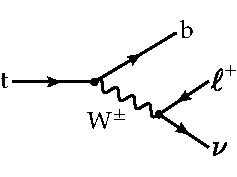
\includegraphics[scale=0.75]{figures/theory/t_decay.pdf}}\hspace{0.15\textwidth}
\subfloat[\label{fig:theory-top-whel-angle}]{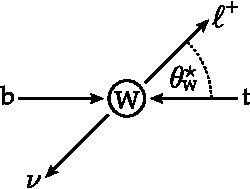
\includegraphics[scale=0.75]{figures/theory/whel.pdf}}
}

The expected distributions per helicity state are presented in Fig.~\ref{fig:theory-whel-distributions} together with the \gls{nnlo} \gls{sm} expectation of $\mathrm{F}_\mathrm{L}=0.311\pm0.005$, $\mathrm{F}_\mathrm{R}=0.0017\pm0.00001$, and $\mathrm{F}_{0}=0.687\pm0.005$~\cite{Czarnecki:2010gb}.

\myfigure{\label{fig:theory-whel-distributions}Distributions of W boson helicity fractions. The \gls{sm} expectation at \gls{nnlo} is taken from Ref.~\cite{Czarnecki:2010gb}.}{
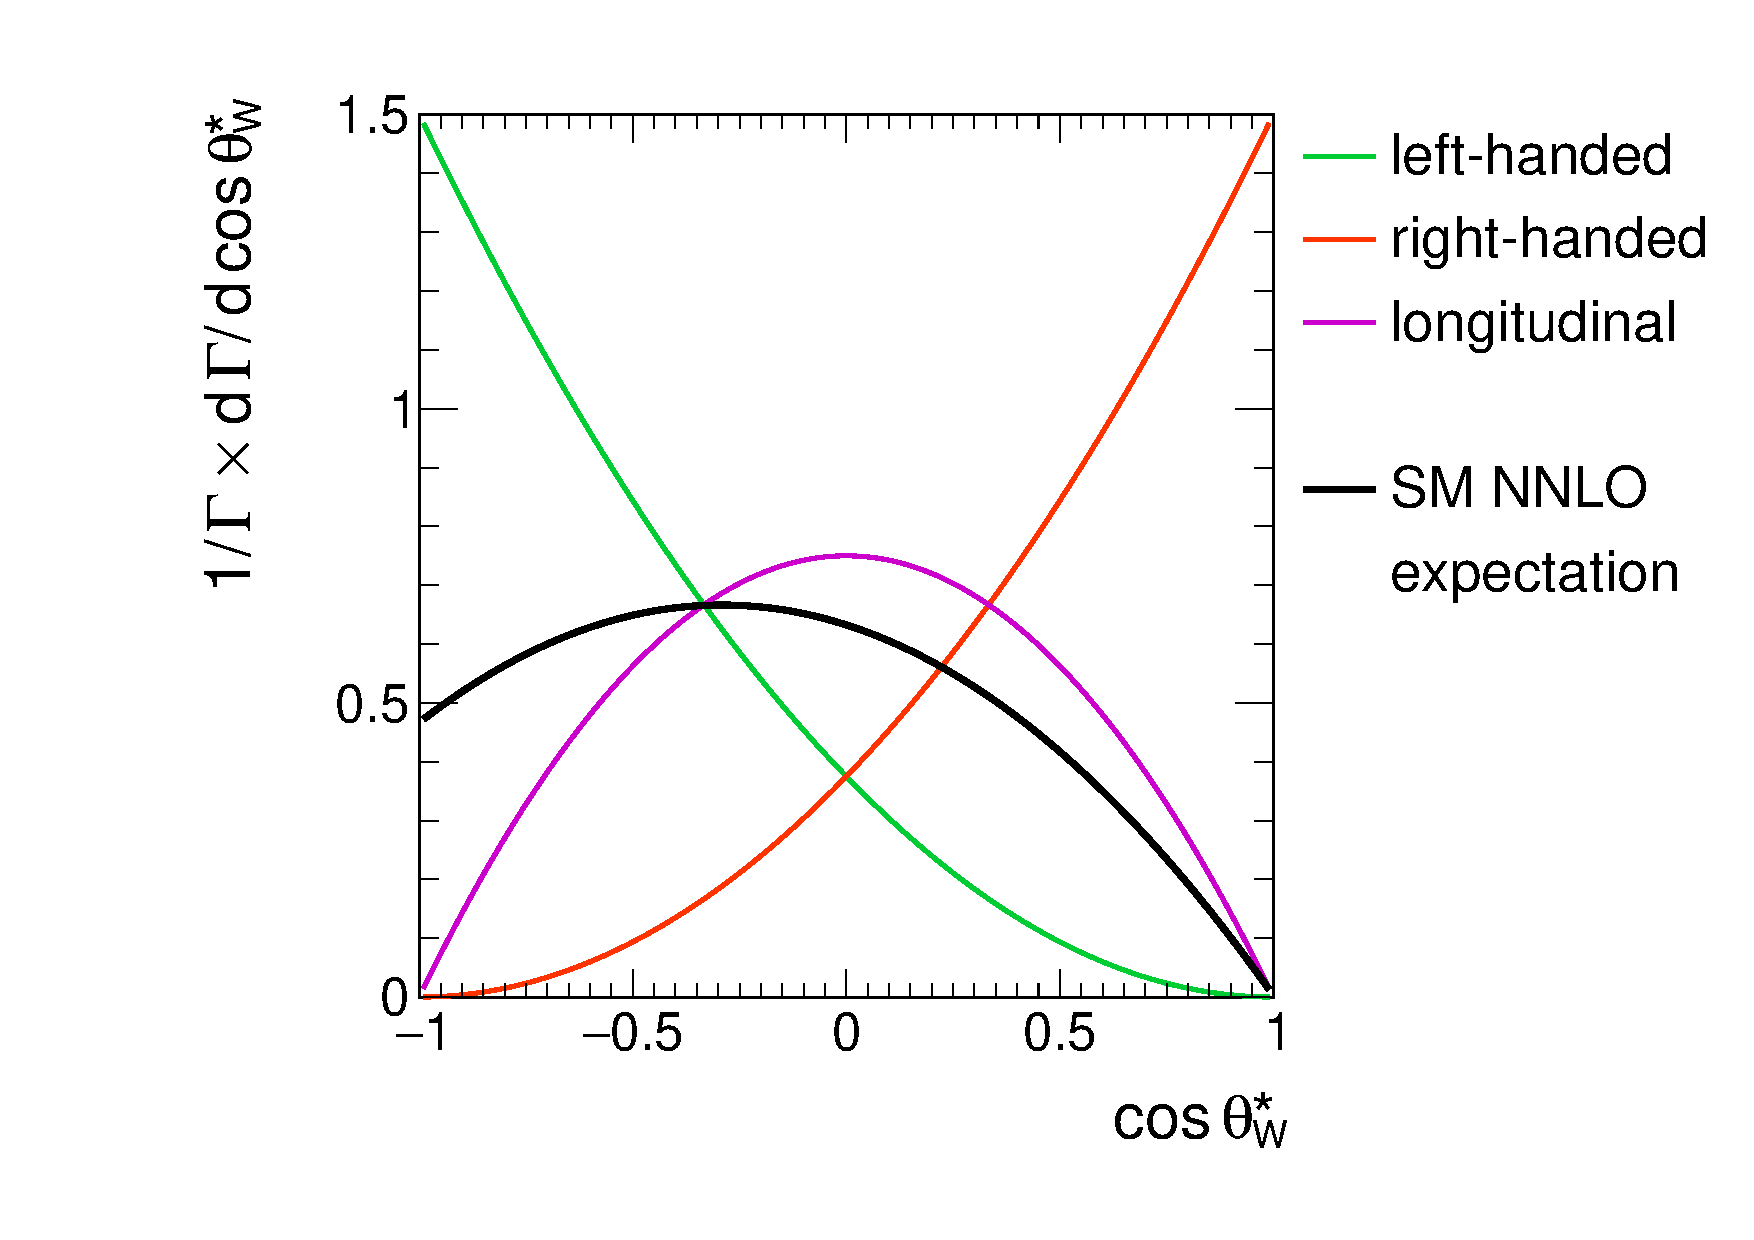
\includegraphics[width=0.49\textwidth]{figures/theory/whel_fractions.pdf}
}

%##############################################
\subsection{Pair production}
%##############################################

The dominant production mechanism at hadron colliders is the production of top quark pairs through strong interactions via gluon or quark fusion. Figure~\ref{fig:theory-feynman-ttbar} shows the corresponding Feynman diagrams at \gls{lo}. \todo{mention gluon fusion leads to high xsec} The top quarks are produced nearly isotropic with only a small net polarization due to electroweak corrections~\cite{Bernreuther:2013aga}. However, their spins are linked yielding a large correlation between them~\cite{Mahlon:2010gw}. 

\myfigure{\label{fig:theory-feynman-ttbar}Feynman diagrams of \ttbar production at \gls{lo}.}{
\subfloat[]{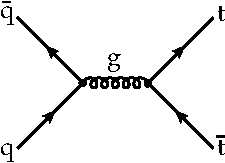
\includegraphics[scale=0.75]{figures/theory/qq2tt_1.pdf}}\hspace{0.03\textwidth}
\subfloat[]{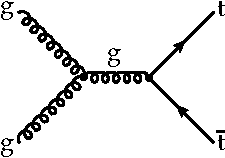
\includegraphics[scale=0.75]{figures/theory/qq2tt_2.pdf}}\hspace{0.03\textwidth}
\subfloat[]{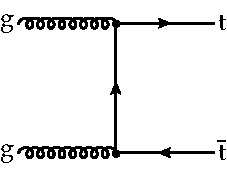
\includegraphics[scale=0.75]{figures/theory/qq2tt_3.pdf}}
}

%##############################################
\subsection{Single top quark production}
%##############################################

The production of single top quarks via electroweak interaction can be characterized into three channels depending on the \wboson boson. Figure~\ref{fig:theory-feynman-singletop} shows the corresponding diagrams at \gls{lo}. The t-channel production mode has the highest cross section in $\mathrm{pp}$ collisions. The second largest is the \wboson-associated production mode. At \gls{nlo} it interferes with \ttbar production which complicates its definition. A recent approach is to combine both production modes and the inference between them into a process with a $\mathrm{WbWb}$ final state~\cite{Cascioli:2013wga}. Lastly, the s-channel is the smallest production mode due to the large virtuality $Q^{2}=-p_{\mu}p^{\mu}$ of the b quark.

\myfigure{\label{fig:theory-feynman-singletop}Feynman diagrams of electroweak single top quark production at \gls{lo} in the 5 flavor scheme.}{
\subfloat[t-channel]{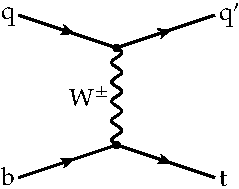
\includegraphics[scale=0.75]{figures/theory/ST_tch.pdf}}\hspace{0.03\textwidth}
\subfloat[tW-channel]{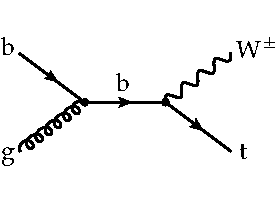
\includegraphics[scale=0.75]{figures/theory/ST_tWch.pdf}}\hspace{0.03\textwidth}
\subfloat[s-channel]{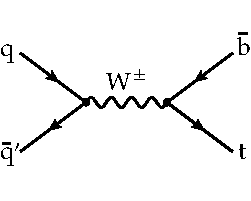
\includegraphics[scale=0.75]{figures/theory/ST_sch.pdf}}
}



xsecs of all top processes, ST supressed by PDFs, t,tW,s channel, exotic production (e.g. tHq, FCNC), decay + coupling structure, Vtb




%##############################################
\subsection{Experimental results}
%##############################################

w helicity results (mention possibility for other polarizations in ST)

ttbar, t,tW,s channel

%##############################################
\subsection{Top quark mass}
%##############################################

vacuum stability, MS bar vs. polemass

%##############################################
\subsection{Flavor schemes}
%##############################################

4vs5

%##############################################
\subsection{Effective operators and anomalous couplings}
%##############################################

decay rates, angles (w polarizations)/spin matrix

EFT (pseudo observables=form factors=e.g. w helicity/polarization?); EFT UV covered models see (https://indico.cern.ch/event/537012/contributions/2371763/attachments/1375462/2088456/talk4.pdf)

